\icode{E-MV-CA-L3-261011-001}
有一列横波，在\(A\)、\(B\)两个质点之间传播，已知\(A\)、\(B\)间距为\qty{3}{m}，\(\lambda >\) \,\qty{3}{m}，其中\(A\)、\(B\)两处质点的振动图像如图所示（实线为\(A\)质点的振动图像）。
\begin{enumerate}
	\item 若这列波是从\(B\)传向\(A\)，求这列波的波长\(\lambda_1\)和波速\(v_1\)；
	\item 若这列波是从\(A\)传向\(B\)，求这列波的波长\(\lambda_2\)和波速\(v_2\)。
\end{enumerate}

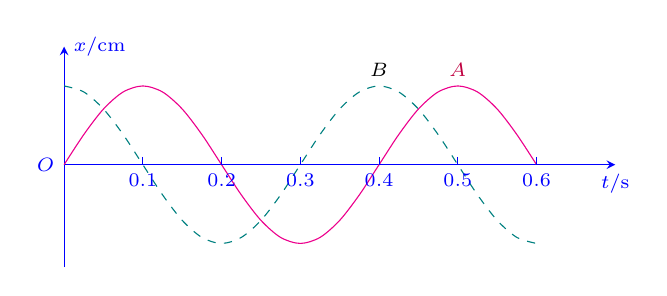
\begin{tikzpicture}[>=stealth,font=\scriptsize]
	\draw[->,blue] (0,-1.3)--(0,1.5)node[right]{\(x\)/\qty{}{cm}};
	\draw[->,blue] (0,0)node[left]{\(O\)}--(7,0)node[below]{\(t\)/\qty{}{s}};
	\draw[domain=0:6,smooth,magenta] plot(\x,{sin(pi*\x/2 r)});
	\draw[domain=0:6,smooth,dashed,teal] plot(\x,{cos(pi*\x/2 r)});
	\foreach \x in {1,2,...,6}
		\draw[blue] (\x,.1)--(\x,0)node[below]{\(0.\x\)};
	\node at(5,1)[above,purple]{\(A\)};
	\node at(4,1)[above]{\(B\)};
\end{tikzpicture}
\begin{answer}
    （1）\(\lambda_1 =\)\,\qty{12}{m}\quad \(v_1 =\)\,\qty{30}{m/s}（2）\(\lambda_2 =\)\,\qty{4}{m}\quad \(v_2 =\)\,\qty{10}{m/s}

    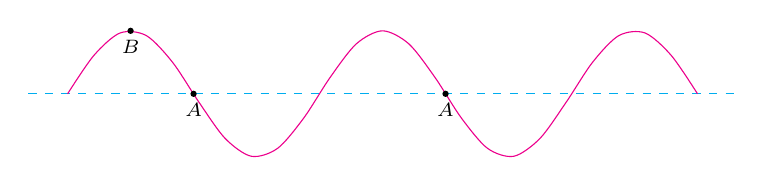
\begin{tikzpicture}[font=\scriptsize]
        \draw[dashed,cyan] (-.5,0)--(8.5,0);
        \draw[domain=0:8,smooth,magenta] plot(\x,{.8*sin(pi*\x/1.6 r)});
        \foreach \c/\str in {(.8,.8)/B,(1.6,0)/A,(4.8,0)/A}
            \fill \c node[below]{\(\str\)} circle(.04);
    \end{tikzpicture}

    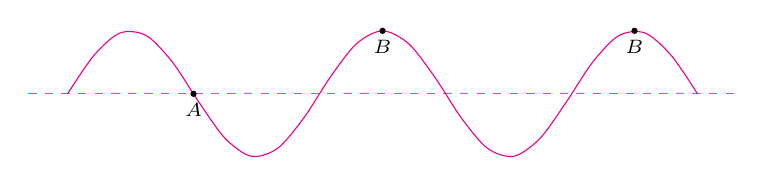
\begin{tikzpicture}[font=\scriptsize]
        \draw[dashed,cyan] (-.5,0)--(8.5,0);
        \draw[domain=0:8,smooth,magenta] plot(\x,{.8*sin(pi*\x/1.6 r)});
        \foreach \c/\str in {(1.6,0)/A,(4,.8)/B,(7.2,.8)/B}
            \fill \c node[below]{\(\str\)} circle(.04);
    \end{tikzpicture}
\end{answer}